% !TEX root = ../main.tex
\section{Trabalho Desenvolvido em Contexto Remoto (Inteligência Artificial e Visão Computacional)}
\label{sec:computacional_ia}

Durante os meses de agosto e setembro de 2026, as atividades prosseguiram em ambiente computacional avançado, com foco na conceção, implementação, treino e validação de um pipeline unificado em Python, PyTorch e OpenCV para processamento de imagem, inteligência artificial profunda e caracterização tridimensional de escoamentos ebulitivos em condutas circulares. O trabalho deu resposta integral ao desafio proposto no concurso \textbf{Capture the Future II}: \emph{<<Desenvolvimento e otimização de um algoritmo de inteligência artificial para reconhecimento e categorização de bolhas num escoamento ebulitivo>>}.

\subsection{Contexto, Desafios Óticos e Objetivos do Desafio CtF II}
\label{subsec:contexto_ia}

A caracterização física de escoamentos bifásicos por videografia de alta velocidade (\emph{High-Speed Video} -- HSV) afigura-se essencial para a compreensão dos mecanismos de nucleação, crescimento, deslizamento, coalescência e destacamento de bolhas. Contudo, em condutas circulares industriais, a extração de dados quantitativos através de visão computacional confronta-se com desafios óticos severos:
\begin{enumerate}
    \item \textbf{Efeito de lente cilíndrica do tubo:} A conduta circular em vidro borossilicato ($D_i = 20{,}0\,\mathrm{mm}$, $D_o = 26{,}0\,\mathrm{mm}$) atua como uma lente cilíndrica convergente espessa perante a retroiluminação colimada. O desfasamento dos índices de refração ($n_{\text{ar}} = 1{,}00 \to n_{\text{vidro}} \approx 1{,}50 \to n_{\text{líquido}} \approx 1{,}33$) concentra a luz numa faixa cáustica central intensa e deflete os raios próximos das paredes, gerando uma subexposição periférica acentuada junto ao bordo superior do canal --- precisamente a região para onde as bolhas e os \emph{slugs} ascendem por forças de impulsão gravítica~\cite{branco2026optical};
    \item \textbf{Reflexo ótico interno nas bolhas (\emph{glare}):} Cada bolha de vapor no seio do líquido atua como uma lente esférica divergente ($n_{\text{líquido}} \approx 1{,}33 \to n_{\text{vapor}} \approx 1{,}00$). Os raios paraxiais atravessam o núcleo gasoso sem desvio substancial, criando um ponto de luz central de intensidade idêntica à do líquido envolvente, enquanto a periferia sofre reflexão total interna originando um contorno escuro. Algoritmos clássicos de limiarização (e.g., Otsu~\cite{otsu1979threshold}) segmentam a bolha erradamente como um toro oco (artefacto de <<donut>>);
    \item \textbf{Ambiguidade de profundidade e desfoque monocular:} O registo bidimensional de uma única câmara projeta um domínio 3D com perda do eixo de visão ($z$). As bolhas fora do plano focal exibem atenuação do gradiente de intensidade na fronteira devido ao desfoque (\emph{defocus blur});
    \item \textbf{Confinamento geométrico cordal:} Na secção transversal circular, a espessura física varia verticalmente segundo o perfil de corda:
    \begin{equation}
        L_{\text{chord}}(y) = 2\sqrt{\max\left(0, \, R_{\text{pipe}}^2 - \Delta y^2\right)}
    \end{equation}
    exigindo modelos volumétricos que respeitem a curvatura real da parede e a conservação da massa.
\end{enumerate}

Para mitigar os artefactos de iluminação, a bancada integrou uma unidade LED traseira de alta intensidade combinada com uma lente cilíndrica corretiva externa especialmente projetada por traçado de raios pelo grupo de investigação~\cite{branco2026optical}, conforme esquematizado na \autoref{fig:diagrama_otica}.

\begin{figure}[!htbp]
    \centering
    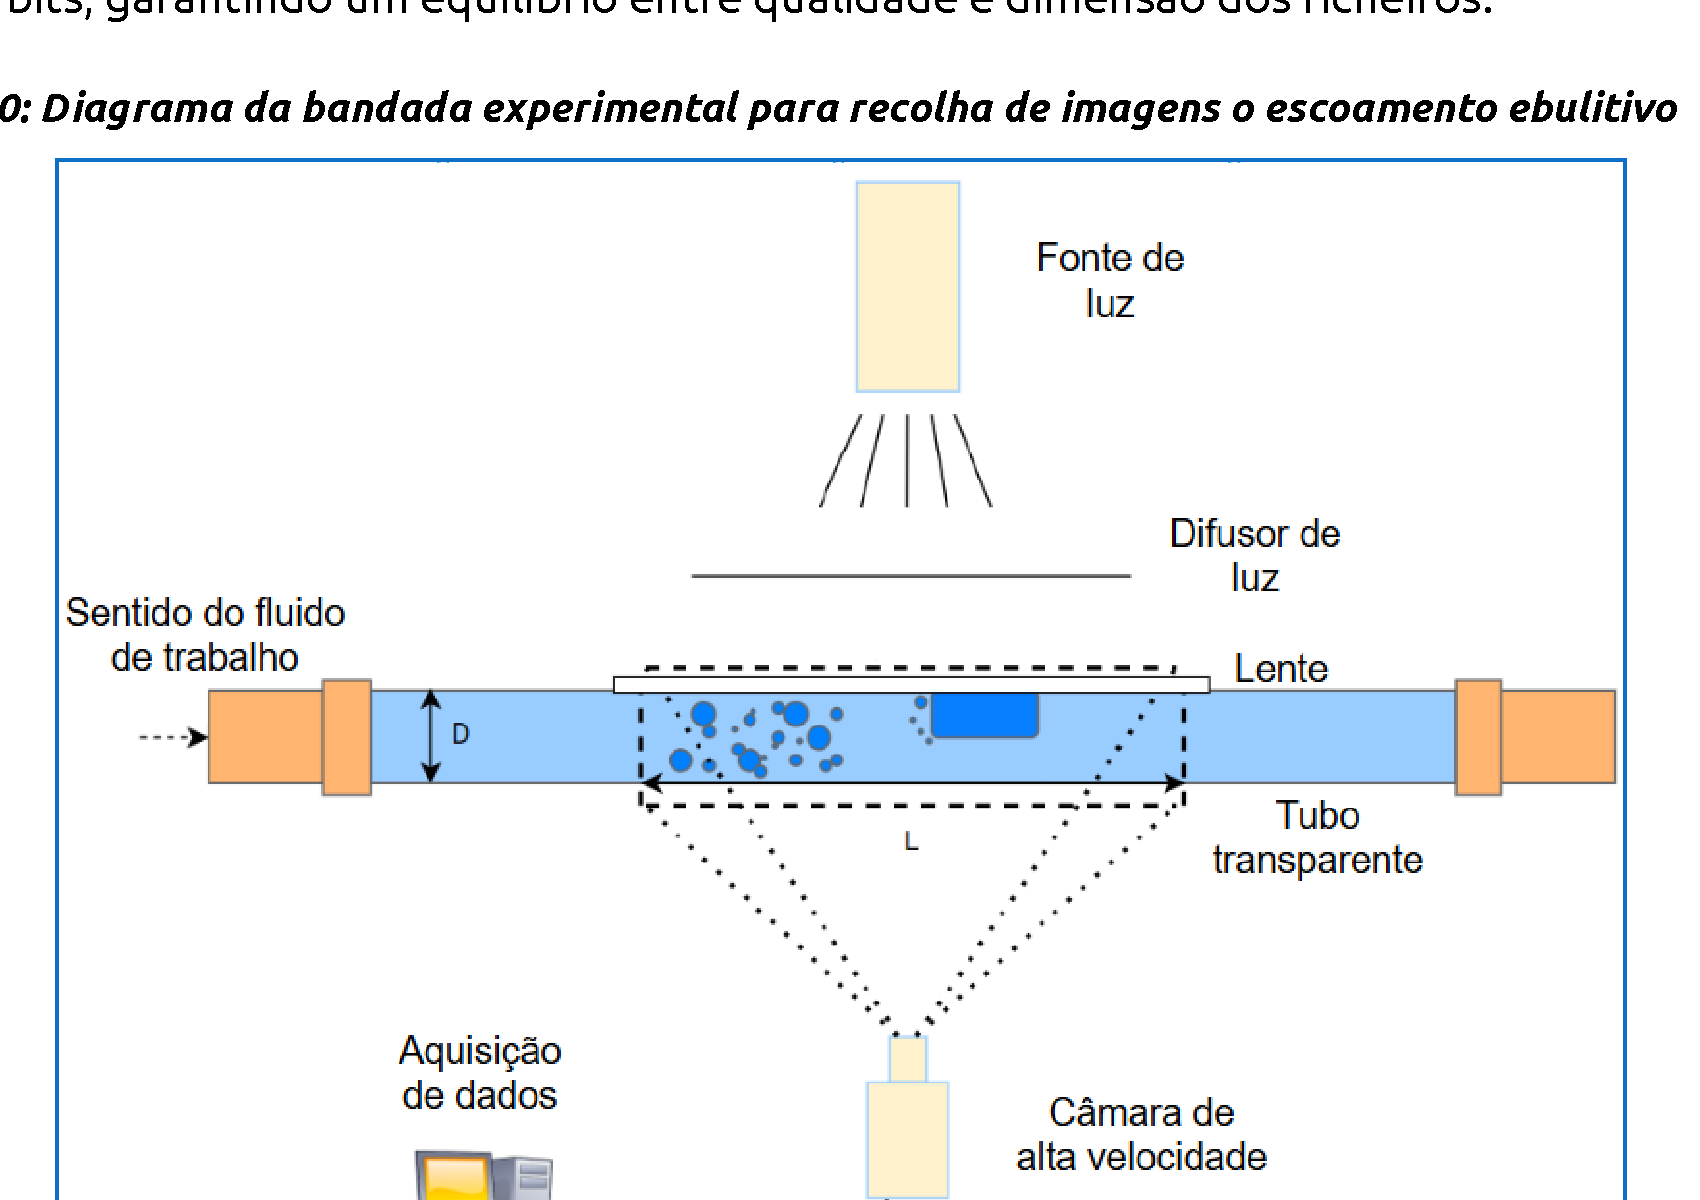
\includegraphics[width=0.85\textwidth]{assets/fig10_diagrama_otica.png}
    \caption{Diagrama esquemático da bancada ótica para aquisição de escoamentos ebulitivos com câmara de alta velocidade e iluminação traseira.}
    \label{fig:diagrama_otica}
\end{figure}

A grandeza macroscópica nuclear a quantificar é a \textbf{fração de vazio} (\emph{void fraction}, $\alpha$), definida como a fração volumétrica ocupada pela fase gasosa no volume de controlo considerado:
\begin{equation}
    \alpha = \frac{V_g}{V_g + V_l} = \frac{V_g}{V_{\text{tubo}}}
    \label{eq:void_fraction_def}
\end{equation}
sendo $V_g$ o volume total tridimensional de gás e $V_{\text{tubo}} = \pi R_{\text{pipe}}^2 W_{\text{FOV}}$ o volume interno da secção cilíndrica monitorizada no campo de visão (\emph{Field of View} -- FOV).

\subsection{Estado da Arte e Inovação da Nova Arquitetura em Python}
\label{subsec:estado_da_arte_ia}

Nos últimos anos, a aplicação de redes neuronais convolucionais baseadas na arquitetura U-Net~\cite{ronneberger2015unet} revolucionou a análise de bolhas em escoamentos térmicos. Seong et al.~\cite{seong2023automated} (MIT) aplicaram uma U-Net clássica com \emph{transfer learning} a bolhas em ebulição subarrefecida em placas planas a 10\,000~FPS, combinando-a com fluxo ótico global de Horn--Schunck~\cite{hornschunck1981}. Passoni et al.~\cite{passoni2024integrating} utilizaram redes convolucionais para estimar a fração de vazio em canais corrugados. Numa abordagem preliminar desenvolvida anteriormente no projeto em MATLAB, utilizou-se uma U-Net otimizada por \emph{Particle Swarm Optimization} (PSO)~\cite{kennedy1995particle}. Contudo, essa implementação inicial apresentava limitações metodológicas e operacionais relevantes:
\begin{itemize}
    \item Dependência do ambiente proprietário MATLAB, com reduzida escalabilidade para processamento em lote e integração de modelos estado-da-arte de visão computacional;
    \item Ausência de conexões residuais no codificador, provocando lentidão na convergência e suscetibilidade à degradação de gradientes durante o \emph{backpropagation};
    \item Utilização exclusiva de funções de perda baseadas em entropia cruzada clássica, vulneráveis ao extremo desequilíbrio entre classes (líquido $>95\%$ da imagem vs. microbolhas gasosas $<5\%$), gerando uma elevada taxa de falsos negativos;
    \item Erro dimensional na formulação da reconstrução volumétrica elipsoidal, onde o semi-eixo de profundidade fora erroneamente definido como a corda total $2\sqrt{R^2-\Delta y^2}$ em vez do semi-eixo de raio $\sqrt{R^2-\Delta y^2}$, introduzindo uma sobrestimação de 100\% no volume das bolhas esferoidais;
    \item Rastreamento cinemático dependente de vizinhos mais próximos gulosos (\emph{greedy}), que colapsava perante rotações, deformações bruscas e eventos de quebra hidrodinâmica (\emph{breakup});
    \item Inexistência de estimativa da coordenada de profundidade fora do plano ($z$).
\end{itemize}

Para superar definitivamente estas restrições, desenvolveu-se em 2026 um ecossistema modular inteiramente em Python, com orquestração centralizada via CLI em \texttt{main.py}. Na \autoref{tab:comparacao_tecnica} sumariza-se o salto qualitativo da nossa abordagem face à literatura e aos scripts exploratórios preliminares em MATLAB desenvolvidos anteriormente no projeto.

\begin{table}[!htbp]
\centering
\small
\caption{Comparação técnica entre abordagens da literatura, baseline preliminar em MATLAB e a nova implementação em Python (2026).}
\label{tab:comparacao_tecnica}
\begin{tabularx}{\textwidth}{>{\raggedright\arraybackslash}p{3.2cm}>{\raggedright\arraybackslash}X>{\raggedright\arraybackslash}X>{\raggedright\arraybackslash}X}
\toprule
\textbf{Característica} & \textbf{Seong et al. (MIT, 2023)} & \textbf{Baseline Preliminar (MATLAB)} & \textbf{Nossa Implementação 2026 (Python)} \\
\midrule
Ambiente \& Framework & Python / TensorFlow & MATLAB Deep Learning & Python 3.12 / PyTorch / OpenCV \\
Codificador (Backbone) & U-Net Clássica (2015) & U-Net Clássica com PSO & \textbf{ResNet-34 Residual (Pré-treinada ImageNet)} \\
Função de Perda & Cross-Entropy pura & Cross-Entropy pura & \textbf{Híbrida: BCE + Dice Loss balanceada} \\
Anotação \& Glare & Contraste básico & Limiarização binarizada & \textbf{Polígonos sólidos (\texttt{fillPoly}), zero donuts} \\
Reconstrução 3D & Área projetada 2D & Extrusão com erro cordal & \textbf{Duplo regime SI ($\mathrm{m}^3$) com confinamento cordal} \\
Rastreio Cinemático & Fluxo Ótico Global & Vizinho Próximo guloso & \textbf{Kuhn--Munkres Húngaro + Quarentena Breakup} \\
Eixo de Profundidade & Inexistente (Plano 2D) & Inexistente (Plano 2D) & \textbf{Depth from Defocus (DFD) com Smoothstep $C^1$} \\
\bottomrule
\end{tabularx}
\end{table}

\subsection{Treino da Rede Neuronal e Otimização}
\label{subsec:treino_unet}

\subsubsection{Arquitetura ResNet-34 U-Net e Função de Perda Híbrida}
\label{subsubsec:unet_arch_loss}

A rede neuronal desenvolvida e treinada neste trabalho baseia-se na arquitetura U-Net~\cite{ronneberger2015unet} dotada de um codificador pré-treinado no repositório ImageNet com blocos residuais de ResNet-34~\cite{he2016deep}, esquematizada na \autoref{fig:unet_arch}. Os blocos residuais com conexões de salto direto (\emph{skip connections}) minoram a degradação de gradientes durante o \emph{backpropagation}, permitindo uma aprendizagem estável e acelerada com convergência rápida mesmo a partir de uma base contendo poucas dezenas de imagens com anotação manual fidedigna ($N \approx 20\text{--}30$ fotogramas representativos gerados via Label Studio com polígonos fechados \texttt{cv2.fillPoly}).

\begin{figure}[!htbp]
    \centering
    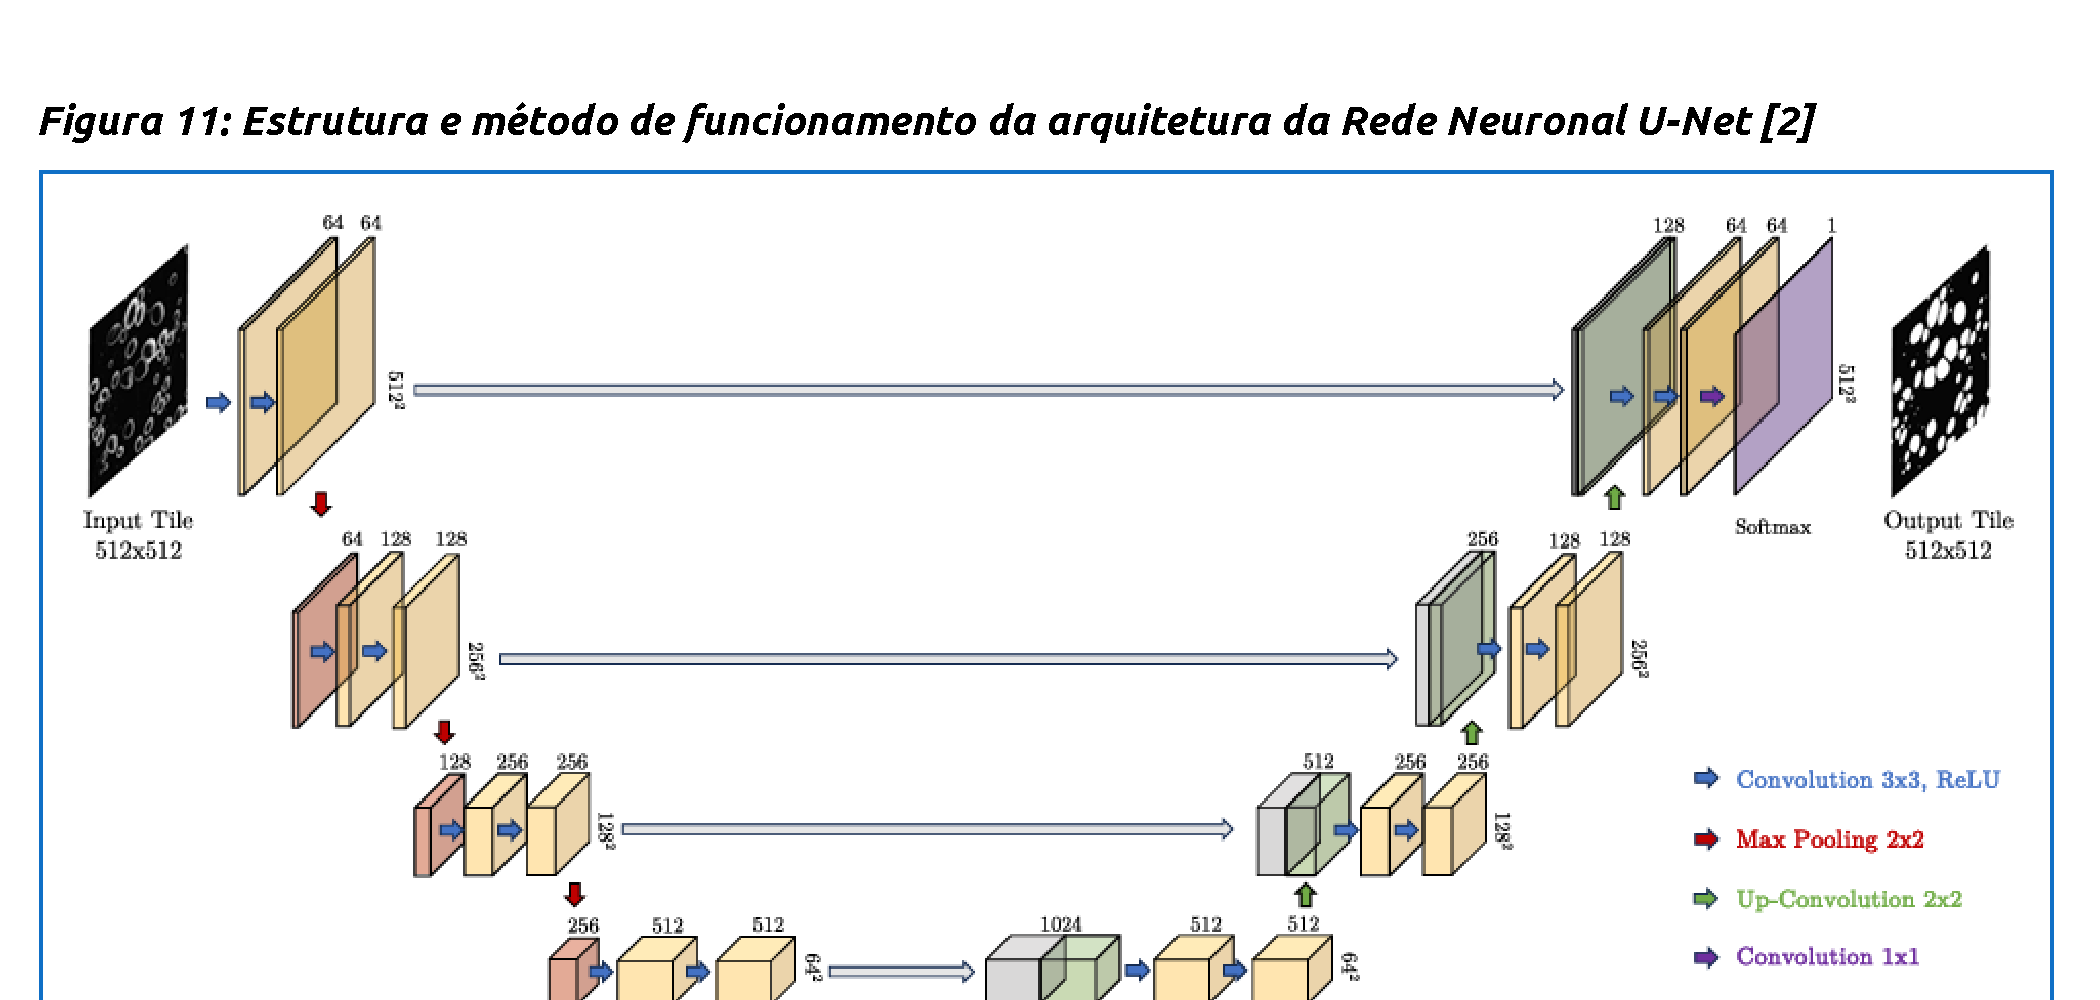
\includegraphics[width=0.92\textwidth]{assets/fig11_unet_arch.png}
    \caption{Arquitetura da rede ResNet-34 U-Net com conexões residuais e perda híbrida para segmentação de bolhas.}
    \label{fig:unet_arch}
\end{figure}

Para mitigar o severo desequilíbrio entre classes típico de regimes ebulitivos dispersos (onde a fase líquida contínua preenche tipicamente mais de 90\% do domínio visual e as microbolhas de vapor representam apenas uma pequena fração dos píxeis), concebeu-se uma função de perda híbrida combinando a Entropia Cruzada Binária ($\mathcal{L}_{\text{BCE}}$) e o Coeficiente de Sobreposição de Dice ($\mathcal{L}_{\text{Dice}}$)~\cite{milletari2016vnet}:
\begin{equation}
    \mathcal{L}_{\text{total}} = \mathcal{L}_{\text{BCE}}(y, \hat{y}) + \mathcal{L}_{\text{Dice}}(y, \hat{y})
    \label{eq:hybrid_loss}
\end{equation}
\begin{equation}
    \mathcal{L}_{\text{BCE}} = -\frac{1}{N_{\text{pix}}} \sum_{p=1}^{N_{\text{pix}}} \left[ y_p \log(\hat{y}_p) + (1 - y_p) \log(1 - \hat{y}_p) \right]
\end{equation}
\begin{equation}
    \mathcal{L}_{\text{Dice}} = 1 - \frac{2 \sum_{p=1}^{N_{\text{pix}}} y_p \hat{y}_p + \epsilon_{\text{smooth}}}{\sum_{p=1}^{N_{\text{pix}}} y_p + \sum_{p=1}^{N_{\text{pix}}} \hat{y}_p + \epsilon_{\text{smooth}}}
\end{equation}
onde $y_p \in \{0, 1\}$ é a máscara real anotada, $\hat{y}_p = \sigma(z_p) \in [0, 1]$ representa a probabilidade sigmoid predita e $\epsilon_{\text{smooth}} = 1{,}0$ denota o termo de regularização suave de Laplace. Ao avaliar a interceção espacial entre as entidades gasosas, a parcela de Dice penaliza fortemente falsos negativos sem permitir que a vasta predominância de verdadeiros negativos na fase líquida mascare a eficácia do modelo.

\subsubsection{Estratégia de Treino e Otimização Hiperparamétrica}
\label{subsubsec:training_strategy}

A otimização dos pesos neuronais foi governada pelo algoritmo AdamW com taxa de aprendizagem inicial de $\eta_0 = 10^{-4}$, decaimento de peso $\lambda_{\text{weight}} = 10^{-2}$ e escalonamento por agendamento de cosseno amortecido (\emph{Cosine Annealing Learning Rate}). Com vista a prevenir a sobremororização (\emph{overfitting}) e dotar a rede de invariância a reflexos luminescentes parasitas, empregou-se uma rotina avançada de aumento artificial de dados (\emph{data augmentation}) através da biblioteca Albumentations: rotações angulares aleatórias ($\pm 15^\circ$), inversões especulares horizontais e verticais, modulações subtis de gama e contraste ($\pm 10\%$) simulando oscilações térmicas da lâmpada halogénea e adição controlada de ruído gaussiano. O procedimento de treino atingiu a convergência ótima ao fim de 40 épocas, ativando o mecanismo de paragem antecipada com base no índice IoU de validação.

\subsubsection{Validação do Modelo, Métricas de Desempenho e Matriz de Confusão}
\label{subsubsec:validation_metrics}

A quantificação do poder preditivo do modelo foi efetuada através do módulo \nolinkurl{evaluate_unet_metrics.py} sobre um conjunto de teste totalmente segregado do treino. Os parâmetros globais de desempenho são discriminados na \autoref{tab:metricas_unet}.

\begin{table}[!htbp]
\centering
\small
\caption{Métricas de desempenho da rede ResNet-34 U-Net no conjunto de teste independente.}
\label{tab:metricas_unet}
\begin{tabularx}{\textwidth}{lcr>{\raggedright\arraybackslash}X}
\toprule
\textbf{Métrica de Avaliação} & \textbf{Valor Absoluto} & \textbf{Percentagem} & \textbf{Significado Físico / Algorítmico} \\
\midrule
Exatidão (\emph{Accuracy}) & $0{,}9499$ & $94{,}99\%$ & Proporção global de píxeis corretamente previstos \\
Precisão (\emph{Precision}) & $0{,}9794$ & $97{,}94\%$ & Pureza das predições gasosas (reduzidos falsos positivos) \\
Sensibilidade (\emph{Recall}) & $0{,}9025$ & $90{,}25\%$ & Capacidade de identificar a totalidade das bolhas reais \\
Especificidade (\emph{Specificity}) & $0{,}9857$ & $98{,}57\%$ & Rigor na classificação da fase líquida contínua \\
\textbf{F1-Score / Coeficiente Dice} & $\mathbf{0{,}9394}$ & $\mathbf{93{,}94\%}$ & Média harmónica entre Precisão e Sensibilidade \\
\textbf{Índice de Jaccard (IoU)} & $\mathbf{0{,}8857}$ & $\mathbf{88{,}57\%}$ & Grau de sobreposição espacial direta entre conjuntos \\
Coeficiente de Matthews (MCC) & $0{,}8990$ & $0{,}8990$ & Correlação balanceada entre classes (escala $-1$ a $+1$) \\
\midrule
Verdadeiros Positivos ($TP$) & \multicolumn{2}{c}{$340\,267$ píxeis} & Fase gasosa corretamente classificada \\
Verdadeiros Negativos ($TN$) & \multicolumn{2}{c}{$492\,551$ píxeis} & Fase líquida corretamente classificada \\
Falsos Positivos ($FP$) & \multicolumn{2}{c}{$7\,159$ píxeis} & Fundo classificado erradamente como bolha \\
Falsos Negativos ($FN$) & \multicolumn{2}{c}{$36\,767$ píxeis} & Regiões de bolha omitidas pelo modelo \\
\bottomrule
\end{tabularx}
\end{table}

Na \autoref{fig:segmentation_comparison} apresenta-se um exemplo de segmentação, onde se comprova que mesmo sob presença de reflexos óticos internos e causticas no vidro, a rede prevê contornos fechados, nítidos e consistentes.

\begin{figure}[!htbp]
    \centering
    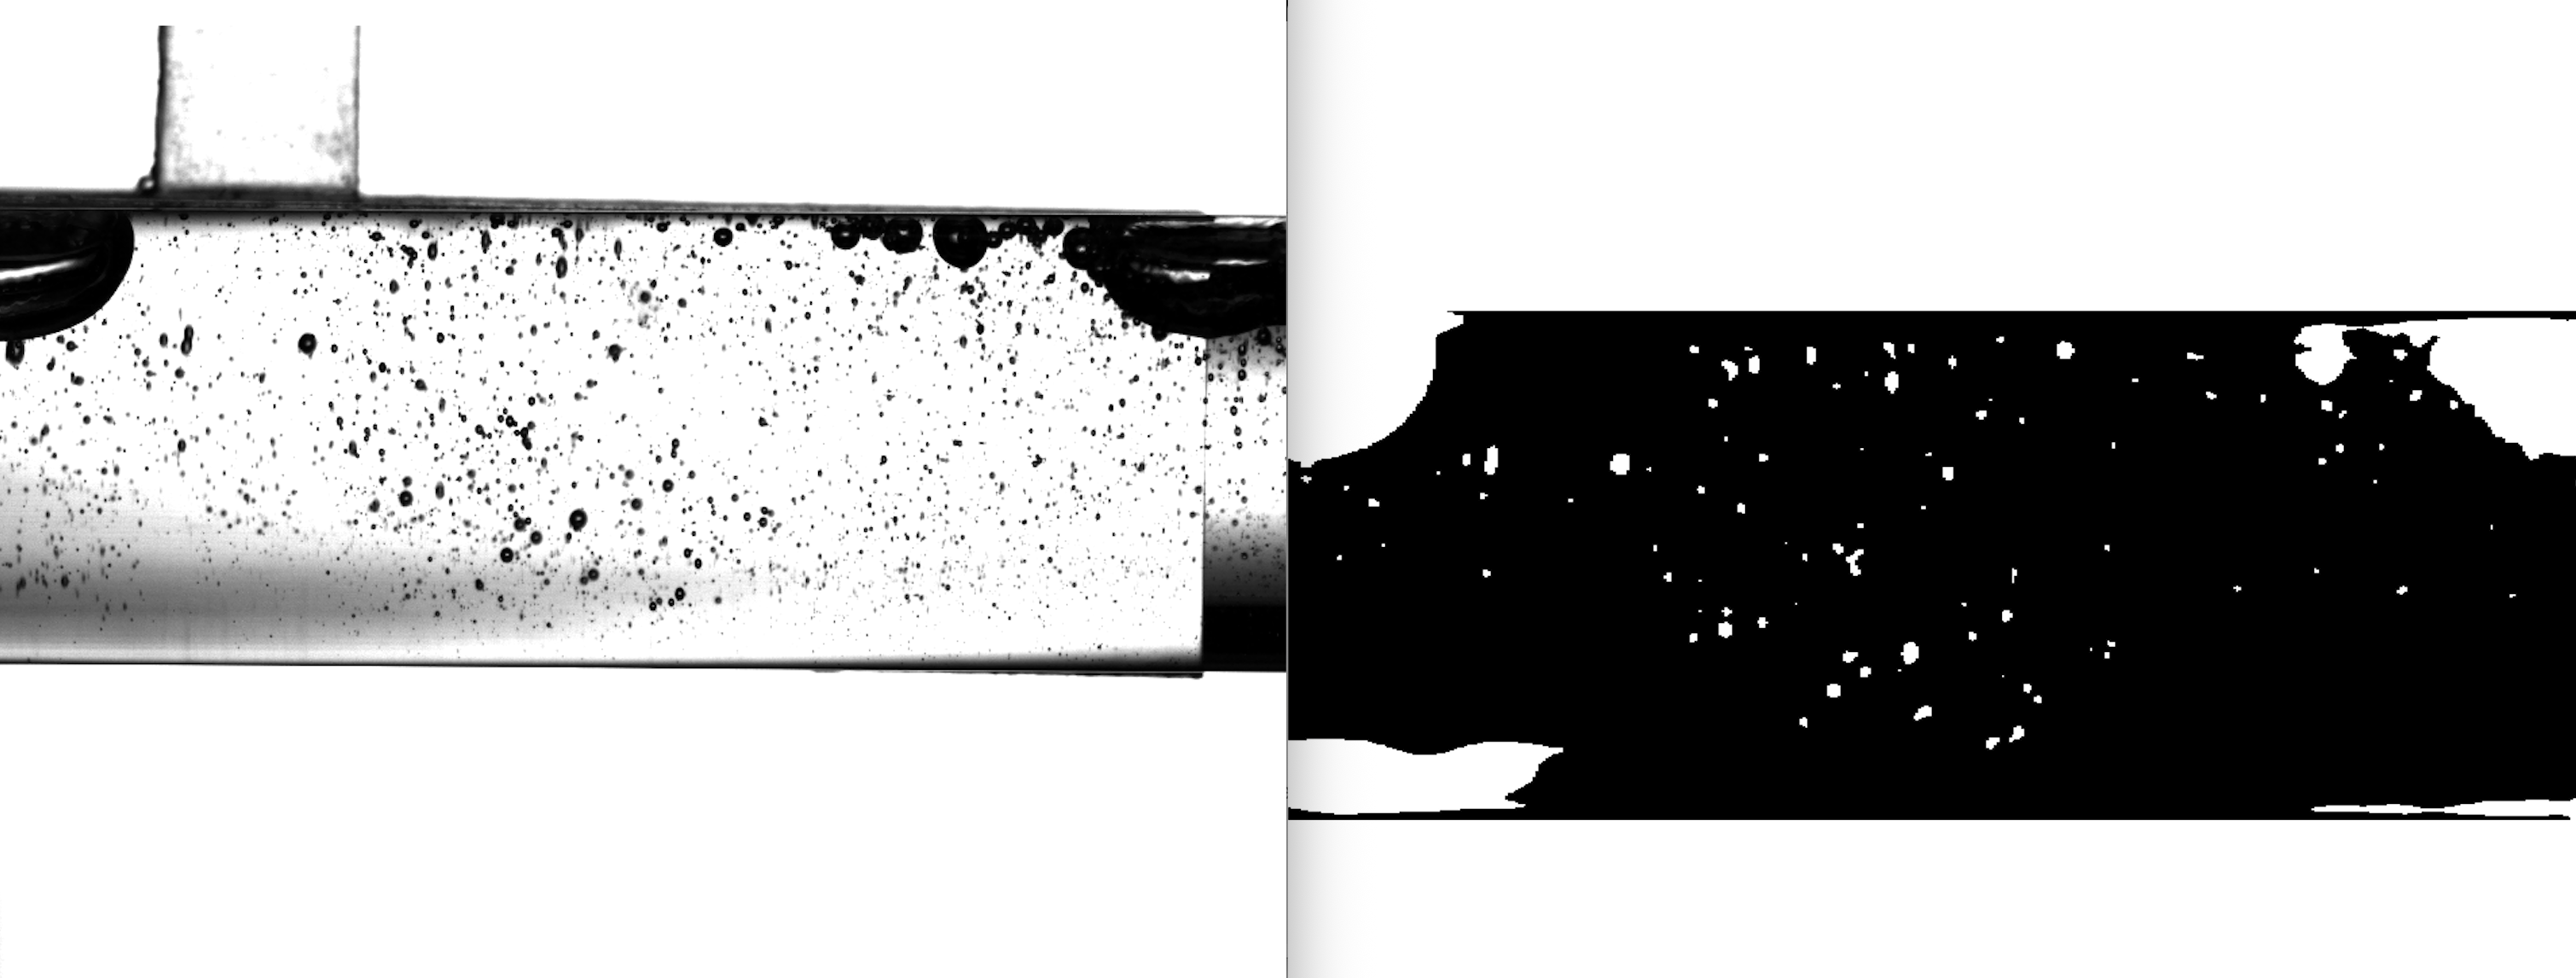
\includegraphics[width=0.92\textwidth]{assets/fig_segmentation_comparison.png}
    \caption{Comparação direta entre o fotograma experimental bruto em tons de cinzento (esquerda) e a máscara binária sólida gerada pelo modelo ResNet-34 U-Net (direita).}
    \label{fig:segmentation_comparison}
\end{figure}

\subsection{Reconstrução Volumétrica Tridimensional de Duplo Regime}
\label{subsec:reconstrucao_3d}

\subsubsection{Pré-Processamento Ótico, Calibração Métrica e Subtração de Fundo}
\label{subsubsec:pre_processing}

A determinação volumétrica fidedigna parte do isolamento da secção interior útil do canal com recurso ao script \nolinkurl{roi_crop_pre_processing.py}, suprimindo reflexos exteriores e fixações mecânicas. 

A calibração dimensional entre píxeis e grandezas físicas no Sistema Internacional é executada pelo utilitário \nolinkurl{test_calibration.py}. A partir do diâmetro interior nominal da secção transparente ($D_i = 20{,}0\,\mathrm{mm}$), estabeleceu-se a escala espacial rigorosa de $s_{\text{px}} = 8{,}60 \times 10^{-5}\,\mathrm{m/px}$ ($86{,}0\,\mu\mathrm{m/pixel}$) para a campanha de alta velocidade analisada. O procedimento de calibração métrica e deteção de interfaces é demonstrado na \autoref{fig:calibracao_pixel}.

\begin{figure}[!htbp]
    \centering
    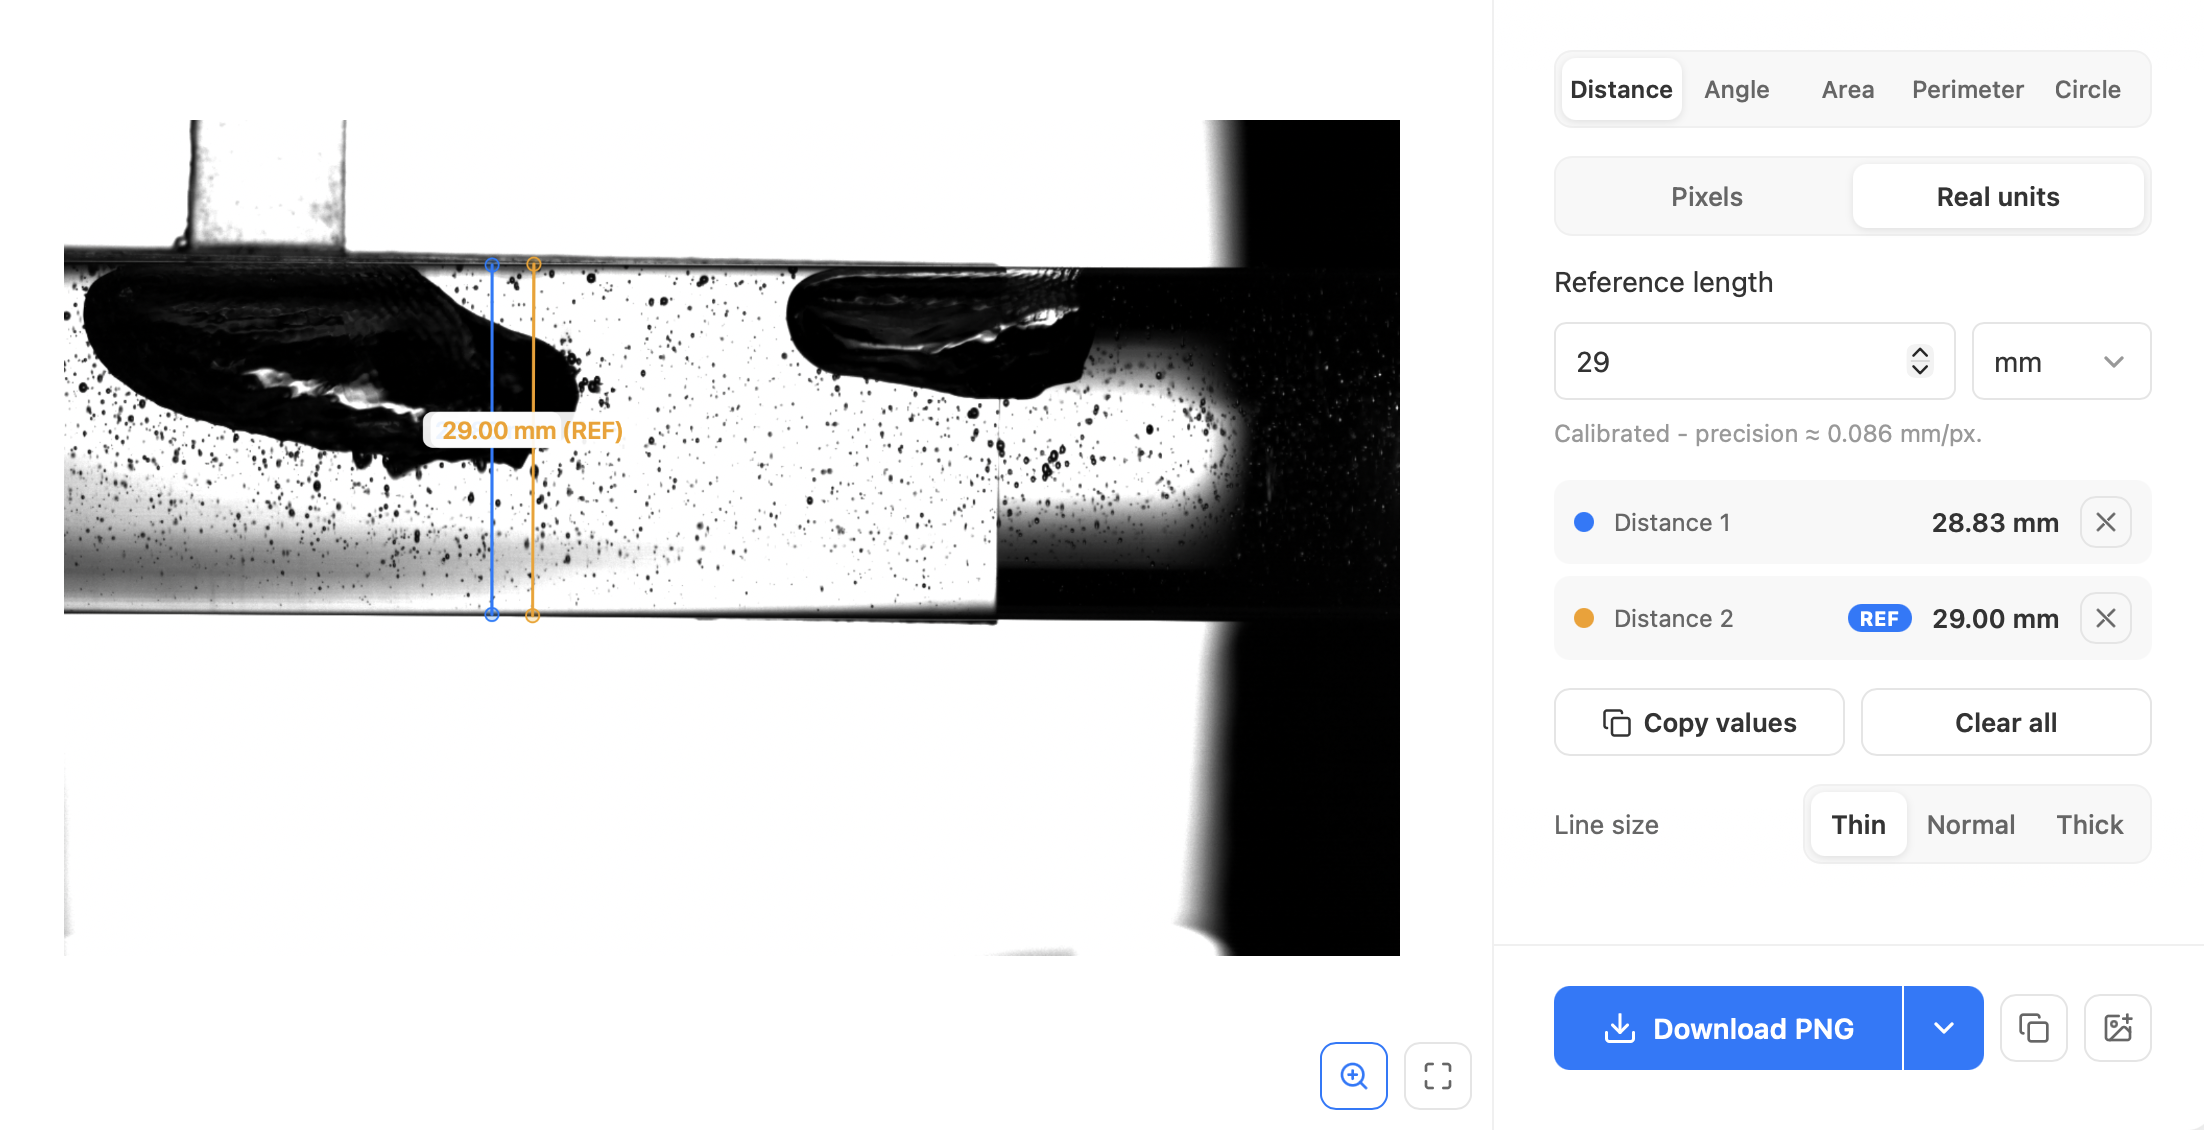
\includegraphics[width=0.88\textwidth]{assets/fig_calibracao_pixel.png}
    \caption{Interface de calibração métrica entre o diâmetro físico do canal ($20{,}0\,\mathrm{mm}$) e a resolução em píxeis.}
    \label{fig:calibracao_pixel}
\end{figure}

De modo a viabilizar a extração precisa de perfis de intensidade e desfoque, implementou-se em \nolinkurl{image_scripts/0_background_subtraction.py} uma rotina de subtração de fundo assente na aquisição de uma imagem de referência monofásica de líquido puro $I_{\text{bg}}(x, y)$, obtida sob idêntica pressão e caudal:
\begin{equation}
    I_{\text{diff}}(x, y) = \max\left(0, \, I_{\text{bg}}(x, y) - I_{\text{raw}}(x, y)\right)
\end{equation}
\begin{equation}
    I_{\text{norm}}(x, y) = \frac{I_{\text{diff}}(x, y)}{\max_{(x,y)} I_{\text{diff}}(x, y) + \varepsilon}
\end{equation}
mantendo-se uma margem de proteção morfológica de 5 píxeis em torno das fronteiras para preservar os gradientes interfaciais. Investigou-se e refutou-se a hipótese de sintetizar o fundo por mediana temporal, uma vez que em regimes de ebulição com escoamento horizontal os grandes \emph{slugs} residem permanentemente na geratriz superior da conduta devido ao empuxo, o que conduziria à inclusão indevida de sombras de vapor no fundo estático gerado.

\subsubsection{Regime 1: Bolhas Pequenas e Elipsoides Confinados}
\label{subsubsec:regime1_bolhas}

A passagem de silhuetas 2D a volumes tridimensionais físicos ($V_g$) assenta num modelo de duplo regime governado pela área de transição $A_{\text{thresh}} = \pi R_{\text{pipe}}^2$.

Para bolhas dispersas de diâmetro inferior ao raio do canal ($A_{\text{proj}} < A_{\text{thresh}}$), assume-se a geometria de elipsoides triaxiais $(a, b, c)$. Os semi-eixos no plano de visualização $xy$ ($a$ e $b$) são determinados por ajuste algébrico direto de mínimos quadrados segundo Fitzgibbon et al.~\cite{fitzgibbon1999direct}. Nos casos em que irregularidades morfológicas induzem sobrestimação de $\pi a b$, aplica-se um fator de escala de conservação estrita de área:
\begin{equation}
    \gamma = \min\left(1{,}0, \, \sqrt{\frac{A_{\text{proj}}}{\pi a b}}\right), \qquad a \leftarrow \gamma \cdot a, \quad b \leftarrow \gamma \cdot b
\end{equation}

O semi-eixo de profundidade ($c$) ao longo do eixo de visão é restringido pela geometria cilíndrica da conduta à coordenada transversal vertical $y_c$:
\begin{equation}
    c = \min\left(b, \, c_{\max}(y_c)\right) = \min\left(b, \, \sqrt{R_{\text{pipe}}^2 - (y_c - y_0)^2}\right)
\end{equation}
resultando no volume elipsoidal:
\begin{equation}
    V_{\text{small}, i} = \frac{4}{3} \pi a b c
\end{equation}
Esta formulação corrige o erro dimensional verificado nos scripts exploratórios preliminares em MATLAB (nos quais constava $c = 2\sqrt{R^2-\Delta y^2}$), prevenindo qualquer violação física da parede sólida do tubo. A \autoref{fig:reconstrucao_frame16} ilustra a correspondência entre a imagem 2D e os elipsoides 3D reconstituídos.

\begin{figure}[!htbp]
    \centering
    \begin{subfigure}[b]{0.48\textwidth}
        \centering
        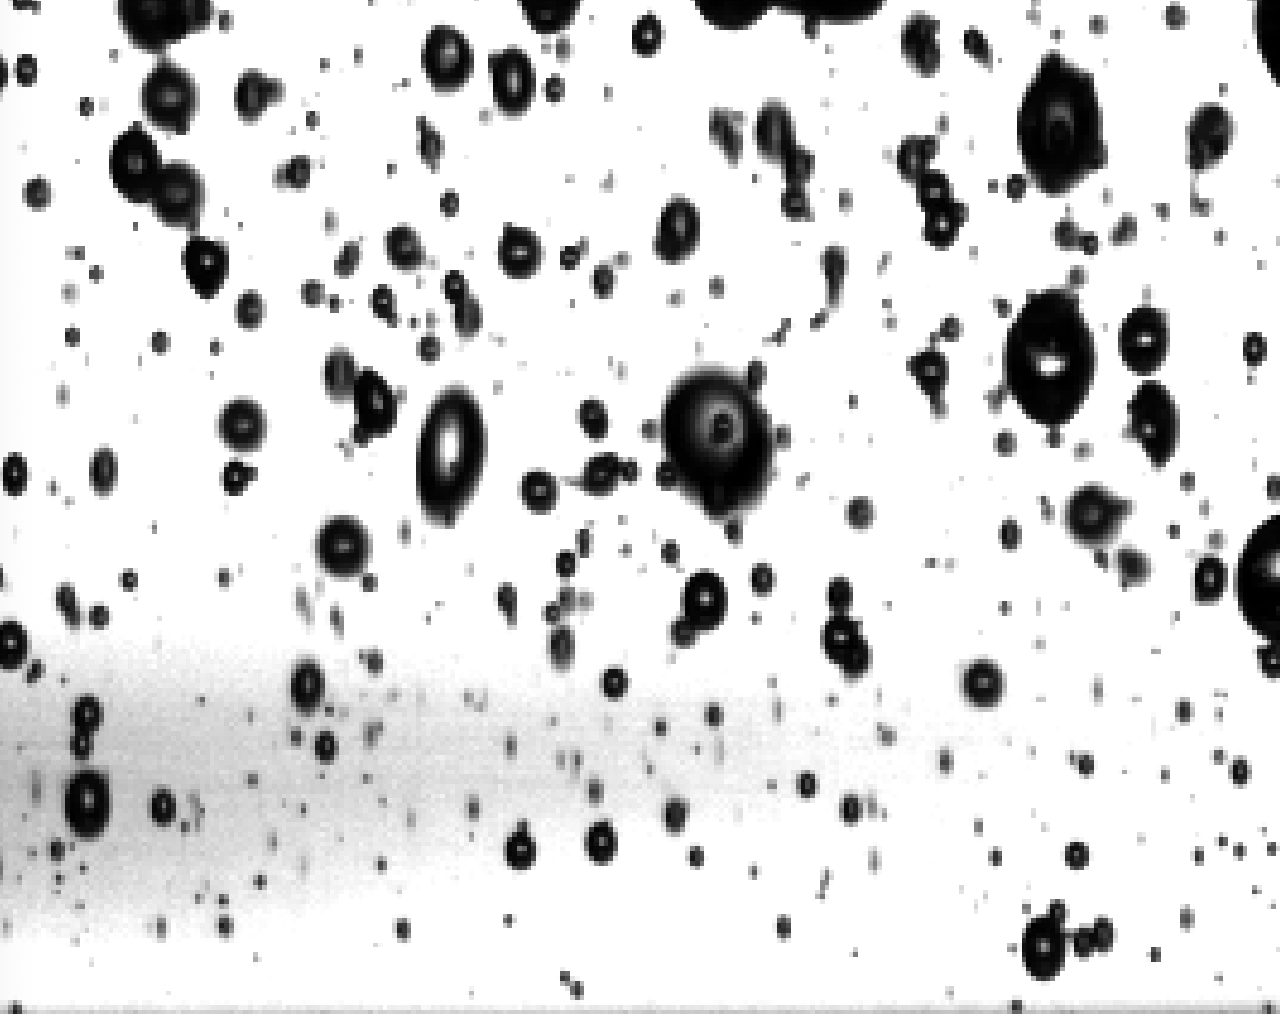
\includegraphics[width=\linewidth]{assets/fig_frame16_2d.png}
        \caption{Projeção 2D de alta velocidade.}
        \label{fig:frame16_2d}
    \end{subfigure}
    \hspace{0.02\textwidth}
    \begin{subfigure}[b]{0.48\textwidth}
        \centering
        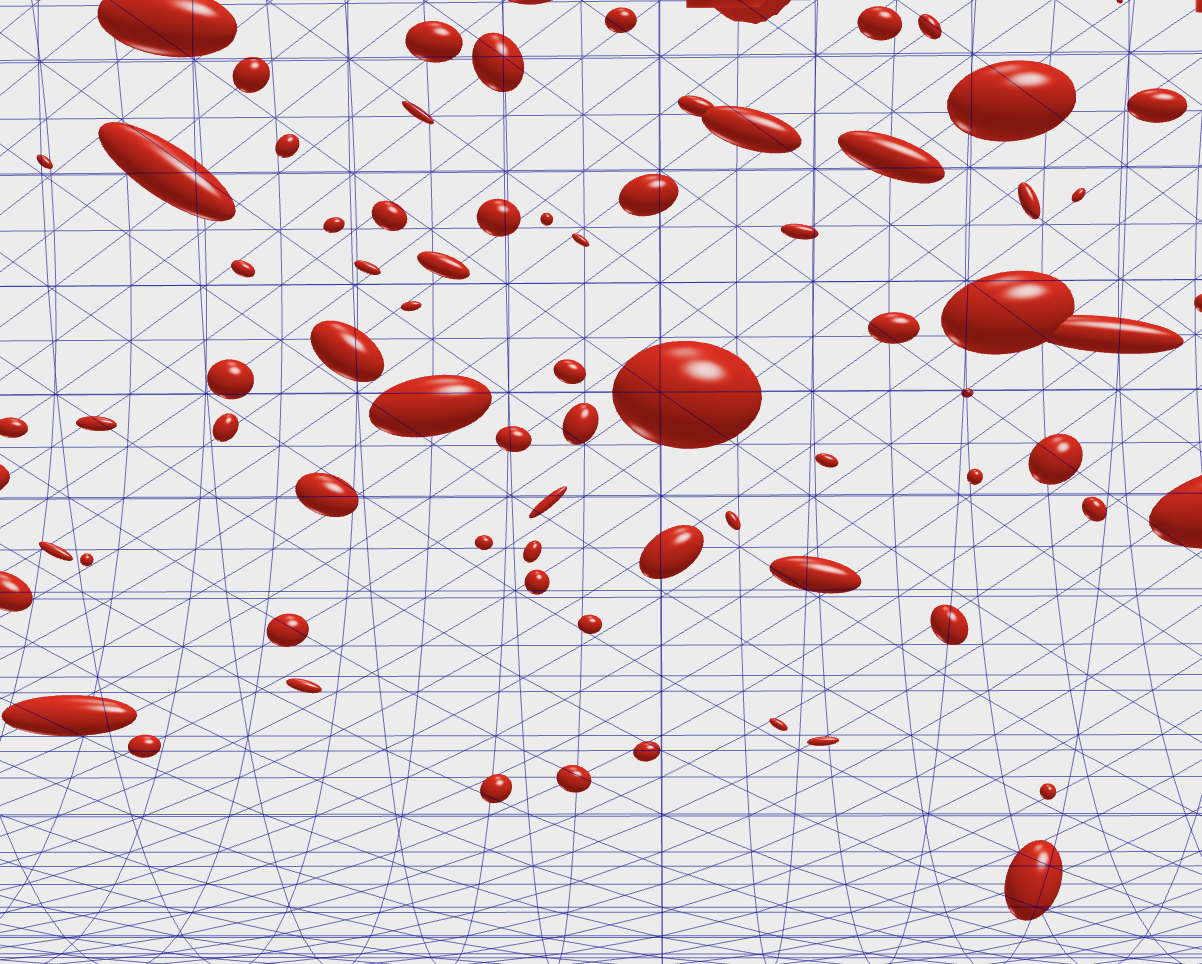
\includegraphics[width=\linewidth]{assets/fig_frame16_3d.png}
        \caption{Reconstrução elipsoidal 3D cordal.}
        \label{fig:frame16_3d}
    \end{subfigure}
    \caption{Visualização comparativa da reconstrução tridimensional no Regime 1 (bolhas pequenas dispersas sob confinamento cordal).}
    \label{fig:reconstrucao_frame16}
\end{figure}

\subsubsection{Regime 2: Grandes Slugs Deformados e Extrusão Bounded por EDT}
\label{subsubsec:regime2_slugs}

Para bolhas de grandes dimensões ou \emph{slugs} ($A_{\text{proj}} \ge A_{\text{thresh}}$) com deformação substancial ao longo da geratriz do tubo, aplica-se a Transformada de Distância Euclidiana (EDT)~\cite{felzenszwalb2012distance} $d_{\text{phys}}(p) = d(p) \cdot s_{\text{px}}$ sobre a máscara binária interior $\Omega_{\text{slug}}$. O perfil de espessura de extrusão $D'(p)$ é limitado pela corda cilíndrica geométrica local $L_{\text{chord}}(y)$:
\begin{equation}
    D'(p) = L_{\text{chord}}(y) \cdot \exp\left(-\frac{1}{\lambda_{\text{phys}} d_{\text{phys}}(p) + \varepsilon}\right)
\end{equation}
\begin{equation}
    D_{\text{bounded}}(p) = \min\left(D'(p), \, L_{\text{chord}}(y)\right)
\end{equation}
onde $\lambda_{\text{phys}} = \lambda_{\text{px}} / s_{\text{px}} \approx 1{,}7 \times 10^3\,\mathrm{m}^{-1}$ (calibrado a partir de $\lambda_{\text{px}} = 0{,}15\,\mathrm{px}^{-1}$ no modelo auditado). O volume é computado por integração de superfície em unidades SI ($\mathrm{m}^3$):
\begin{equation}
    V_{\text{slug}, i} = s_{\text{px}}^2 \sum_{p \in \Omega_i} D_{\text{bounded}}(p)
\end{equation}

\subsubsection{Cálculo da Fração de Vazio no Volume de Controlo}
\label{subsubsec:void_fraction_calc}

A fração de vazio instantânea $\alpha(t)$ é avaliada com rigor físico em cada instante integrando a totalidade dos volumes gasosos de ambos os regimes no interior do volume de controlo cilíndrico $V_{\text{tubo}} = \pi R_{\text{pipe}}^2 W_{\text{FOV}}$, conforme definido na \autoref{eq:void_fraction_def}. A implementação em unidades estritamente coerentes do Sistema Internacional previne discrepâncias de escala entre fotogramas e diferentes resoluções óticas.

\subsubsection{Visualização Tridimensional e Renderização do Escoamento}
\label{subsubsec:visualizacao_3d}

Para além do cálculo quantitativo, o algoritmo integra rotinas de renderização fotorrealista com malhas 3D texturizadas e mapas de densidade volumétrica. Na \autoref{fig:reconstrucao_3d_cilindrica} e na \autoref{fig:reconstrucao_large_slug} exibem-se as reconstituições tridimensionais geradas, evidenciando o tubo transparente, a coexistência entre bolhas dispersas e macro-slugs, e o respeito integral pelas fronteiras do canal.

\begin{figure}[!htbp]
    \centering
    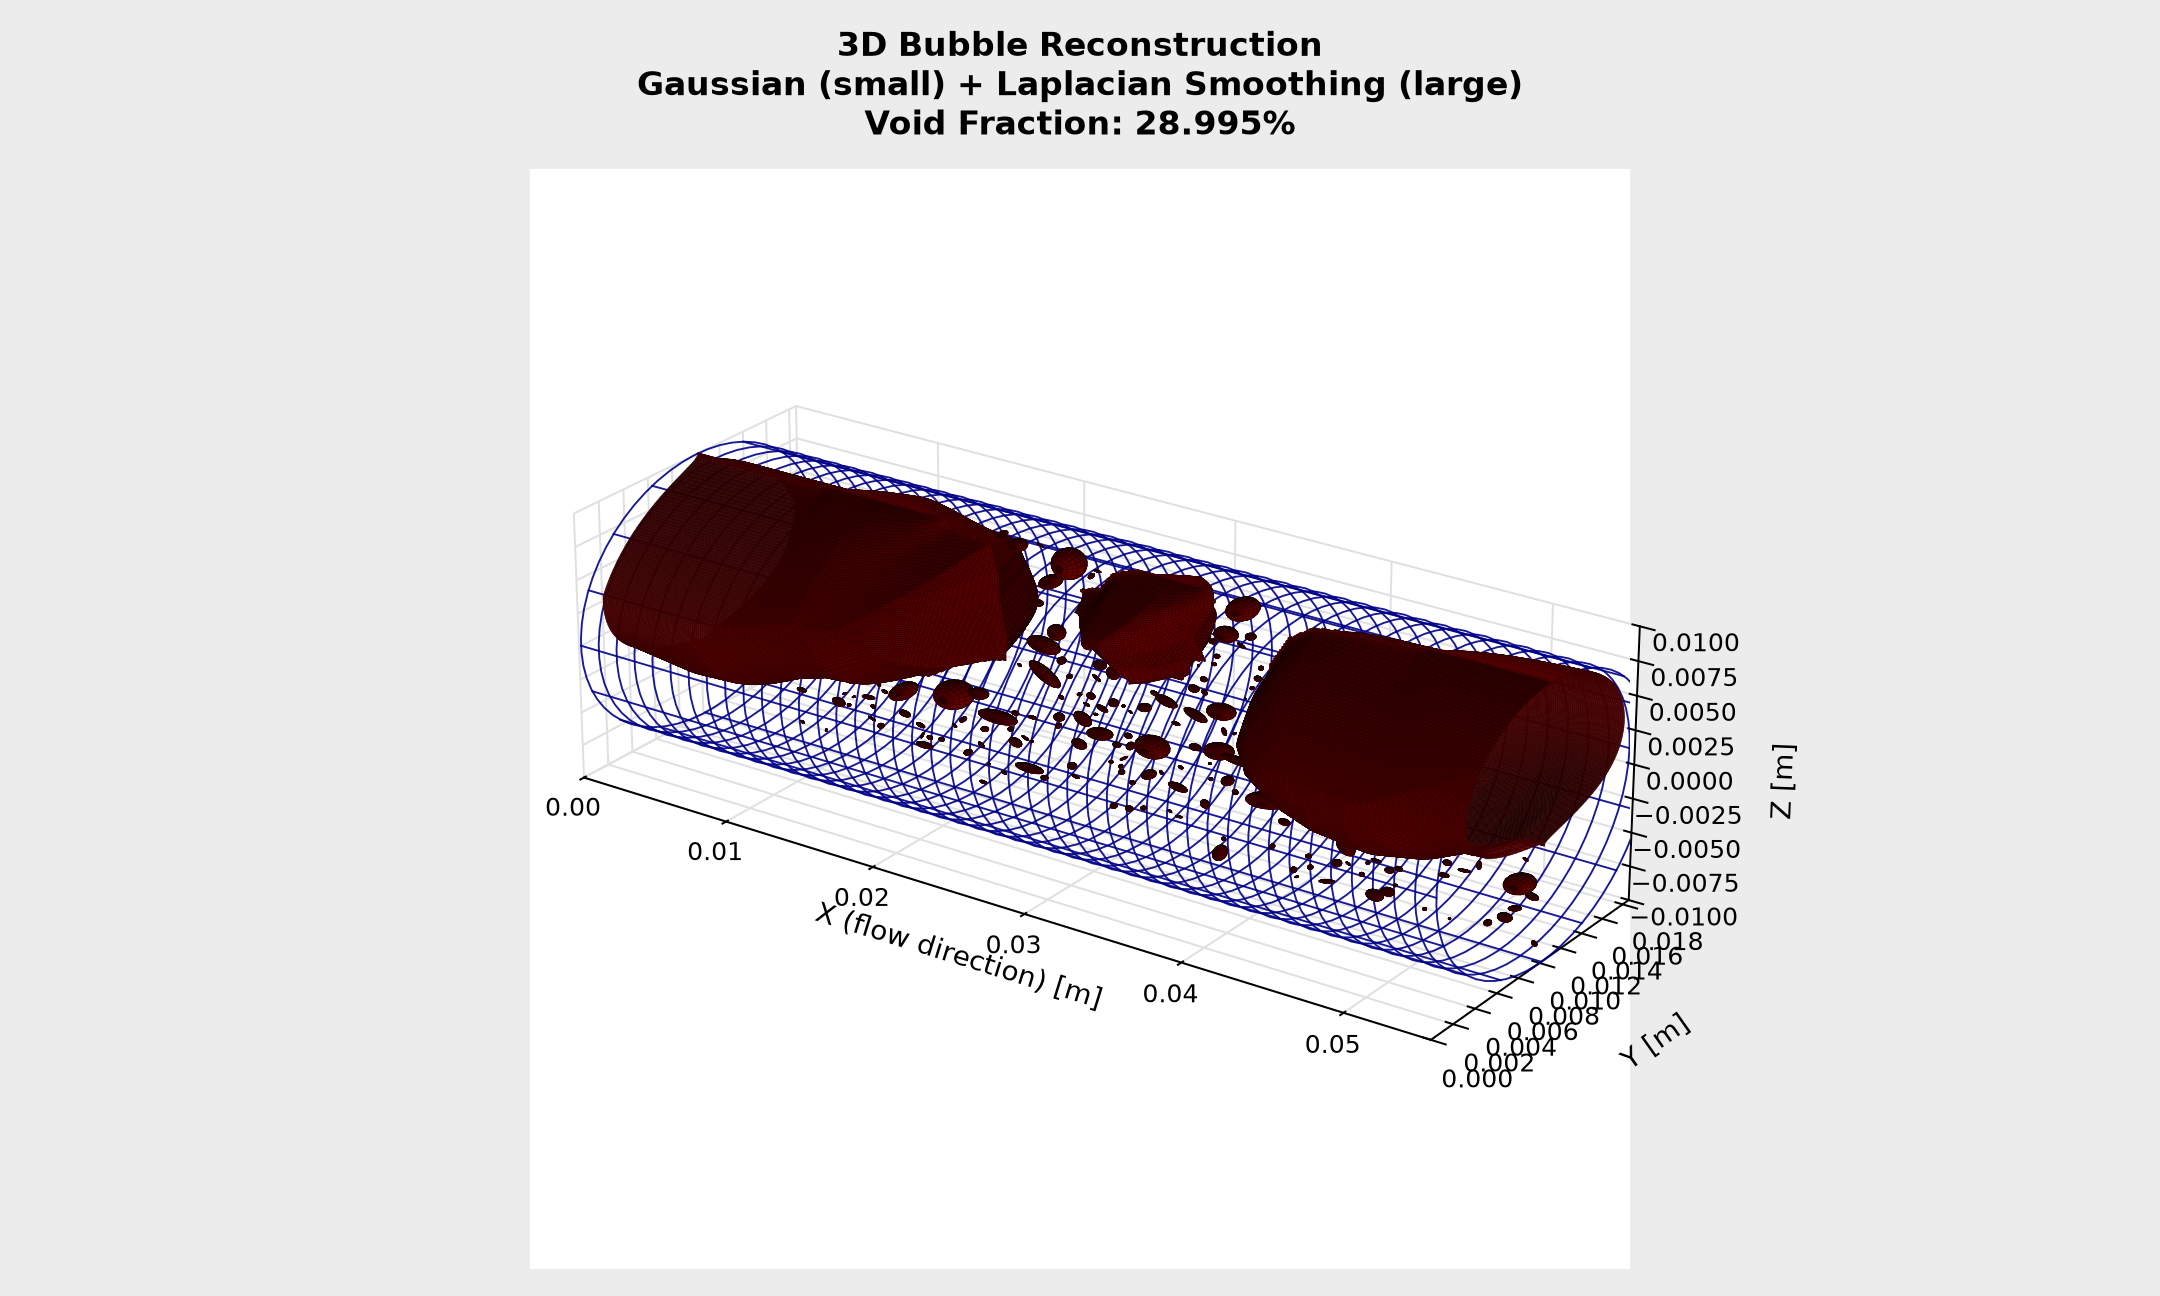
\includegraphics[width=0.92\textwidth]{assets/fig_reconstrucao_3d_cilindrica.png}
    \caption{Reconstrução tridimensional completa do escoamento ebulitivo no interior do canal circular ($D_i = 20\,\mathrm{mm}$), com fração de vazio calculada em unidades SI ($\alpha = 28{,}995\%$).}
    \label{fig:reconstrucao_3d_cilindrica}
\end{figure}

\begin{figure}[!htbp]
    \centering
    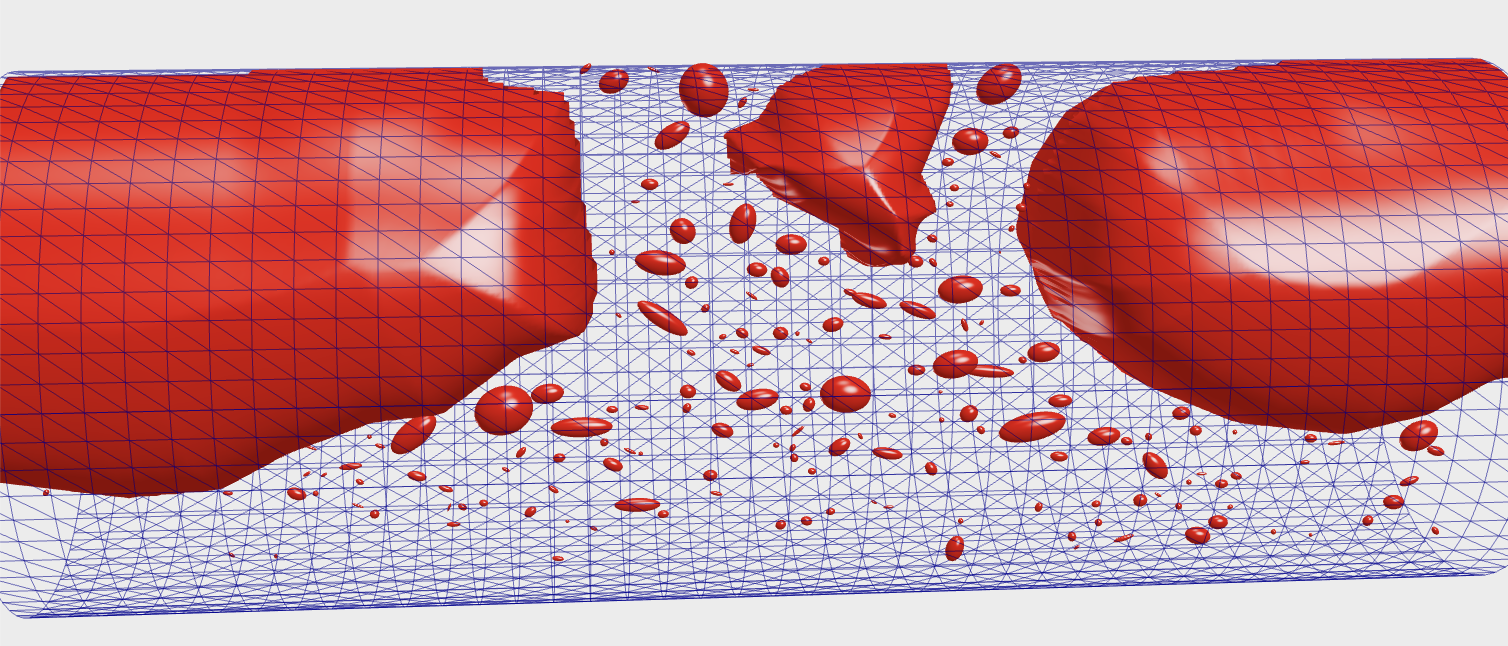
\includegraphics[width=0.88\textwidth]{assets/fig_reconstrucao_large_slug.png}
    \caption{Visualização tridimensional demonstrativa do Regime 2: grande \emph{slug} deformado contíguo à parede superior e balizado pelo perfil de corda $L_{\text{chord}}(y)$.}
    \label{fig:reconstrucao_large_slug}
\end{figure}

\subsection{Análise Sistemática de Séries Temporais a 2000 FPS}
\label{subsec:cinematica_tracking}

\subsubsection{Rastreio Cinemático por Algoritmo Húngaro (Kuhn--Munkres)}
\label{subsubsec:tracking_hungarian}

O acompanhamento temporal das trajetórias das bolhas a $2000\,\mathrm{FPS}$ ($\Delta t = 0{,}5\,\mathrm{ms}$) enfrenta grandes translações no plano ($\Delta x > 20\text{--}50\,\mathrm{px}$), rotações de esteira e fenómenos de corte hidrodinâmico. A associação ótima entre centroides nos instantes consecutivos $t$ e $t+1$ é formalizada como um problema de atribuição bipartida linear ponderada pela distância euclidiana advectada, resolvido de forma exata pelo algoritmo de Kuhn--Munkres~\cite{kuhn1955hungarian, munkres1957algorithms}.

Para cada par com correspondência válida ($d \le d_{\max} = 50\,\mathrm{px}$), o vetor velocidade instantânea $\vec{v}_i = (u_i, v_i)$ é obtido no Sistema Internacional:
\begin{equation}
    u_i(t) = \frac{(x_{\pi(i)}(t+1) - x_i(t)) \cdot s_{\text{px}}}{\Delta t}, \qquad v_i(t) = \frac{(y_{\pi(i)}(t+1) - y_i(t)) \cdot s_{\text{px}}}{\Delta t} \quad [\mathrm{m/s}]
\end{equation}

Na \autoref{fig:flow_tracking_vectors} apresenta-se um fotograma do vídeo vetorial com telemetria HUD instantânea em tempo real, rastreio de centroides e mapa de cores \emph{Turbo} para a magnitude das velocidades.

\begin{figure}[!htbp]
    \centering
    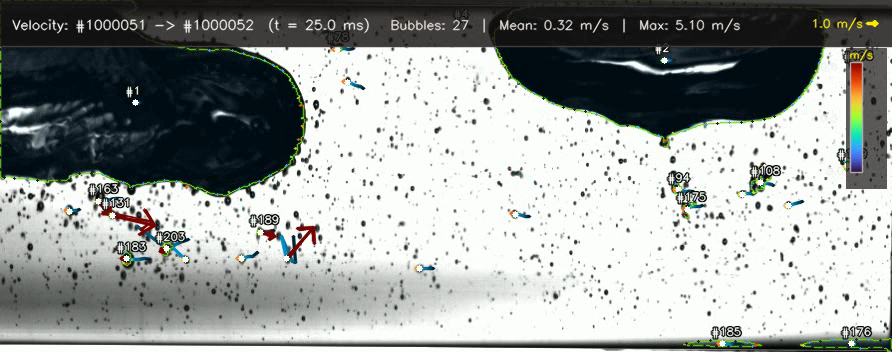
\includegraphics[width=0.95\textwidth]{assets/fig_flow_tracking_vectors.png}
    \caption{Visualização do campo vetorial de velocidades das bolhas com telemetria HUD instantânea a 2000~FPS (velocidade média de $0{,}32\,\mathrm{m/s}$ e pico local de $5{,}10\,\mathrm{m/s}$ na esteira do \emph{slug}).}
    \label{fig:flow_tracking_vectors}
\end{figure}

\subsubsection{Desacoplamento de Fenómenos de Fragmentação e Coalescência}
\label{subsubsec:breakup_quarantine}

Em escoamentos de elevada turbulência, uma bolha mãe pode fragmentar-se em múltiplas bolhas filhas ($1 \to N$), colapsando modelos convencionais de atribuição biunívoca. Para superar esta falha, introduziu-se um estágio de pré-deteção e quarentena de \emph{breakup}:
\begin{enumerate}
    \item Para cada bolha $i$ no fotograma $t$, define-se uma janela de busca advectada com o escoamento médio carrier $\mathcal{W}_i$:
    \begin{equation}
        \mathcal{W}_i = [x_i + \Delta x_{\text{bulk}} - \delta, \, x_i + w_i + \Delta x_{\text{bulk}} + \delta] \times [y_i + \Delta y_{\text{bulk}} - \delta, \, y_i + h_i + \Delta y_{\text{bulk}} + \delta]
    \end{equation}
    \item Surgindo duas ou mais entidades filhas no instante $t+1$ no interior de $\mathcal{W}_i$, avalia-se a conservação de área interfacial:
    \begin{equation}
        \epsilon_{\text{breakup}} = \frac{\left| \sum_{k \in \mathcal{K}_i} A_k(t+1) - A_i(t) \right|}{A_i(t)} \le 0{,}35
    \end{equation}
    \item Verificada a quebra, os índices correspondentes são arquivados no registo físico de eventos (\nolinkurl{bubble_breakups_si.csv}) e colocados em quarentena na matriz de custos com penalização infinita ($C_{ij} \leftarrow 10^4 \cdot d_{\max}$), permitindo que o algoritmo de Kuhn--Munkres atue sobre as bolhas $1$-para-$1$ remanescentes sem gerar falsas velocidades anómalas.
\end{enumerate}

\subsubsection{Determinação de Profundidade por Desfocagem (Depth from Defocus -- DFD)}
\label{subsubsec:dfd_monocular}

Como inovação pioneira face aos relatórios precedentes, formulou-se a adaptação analítica da técnica de \emph{Depth from Defocus} (DFD) monocular~\cite{rao2024depth} ao escoamento em condutas circulares, permitindo a extração da profundidade fora do plano ($z$) e do diâmetro real focado ($d_0$) a partir de uma única câmara ótica, sem necessidade de intrusão física.

Uma bolha de raio focado $r_0$ convoluída com a função de dispersão pontual ótica (PSF) gaussiana com parâmetro de desfoque $\sigma$ produz uma distribuição de intensidade $g_t(r)$. Rao et al.~\cite{rao2024depth} provaram que na fronteira de meia-intensidade ($g_t = 0{,}50$, $r=r_t$), existe uma relação analítica universal e estritamente monótona entre o gradiente de intensidade adimensional $\widetilde{G}$ e o desfoque adimensional $\widetilde{\sigma} = \sigma / d_0$:
\begin{equation}
    \widetilde{G} = \left| r_t \left. \frac{\mathrm{d}g_t}{\mathrm{d}r} \right|_{r=r_t} \right| = f_2(\widetilde{\sigma}), \qquad \widetilde{\rho} = \frac{r_t}{d_0} = f_1(\widetilde{\sigma})
\end{equation}

Ao ancorar o plano focal ótico rigorosamente na parede frontal da conduta em vidro ($z_f \approx 0$), o parâmetro de desfoque cresce linearmente com a profundidade transversal do canal: $\sigma = \beta_{\text{eff}} \cdot z$, com $\beta_{\text{eff}} \approx 2000\,\mathrm{px/m}$ calibrado na montagem ótica, eliminando em absoluto a ambiguidade direcional de sinal (frente vs. trás).

Para filtrar reflexos locais parasitas no contorno da bolha $\mathcal{C}$, aplicou-se um operador de gradiente por média aparada (\emph{trimmed-mean}), descartando os percentis inferior e superior ($P_{15} \le |\nabla I| \le P_{85}$):
\begin{equation}
    \overline{|\nabla I|}_{\text{trimmed}} = \frac{1}{|\mathcal{C}_{\text{valid}}|} \sum_{p \in \mathcal{C}_{\text{valid}}} |\nabla I(p)| \implies \widetilde{G} = r_t \cdot \overline{|\nabla I|}_{\text{trimmed}}
\end{equation}

Para tratar a zona cega próxima do foco (\emph{near-focus blind zone}, $\widetilde{\sigma} < 0{,}05$) onde as bolhas nucleadas deslizam na parede frontal aquecida, introduziu-se uma rampa assintótica cúbica $C^1$-contínua (\emph{smoothstep}):
\begin{equation}
    u = \max\left(0, \, \min\left(1, \, \frac{\widetilde{\sigma}}{\widetilde{\sigma}_{\text{thresh}}}\right)\right), \qquad S(u) = 3u^2 - 2u^3
\end{equation}
\begin{equation}
    \widetilde{\rho}_{\text{reg}} = 0{,}5 \cdot (1 - S(u)) + \widetilde{\rho} \cdot S(u), \qquad d_0 = \frac{2 r_t}{2 \widetilde{\rho}_{\text{reg}}}, \qquad z = \frac{\widetilde{\sigma} d_0 S(u)}{\beta_{\text{eff}}}
\end{equation}
Quando a bolha se aproxima da parede frontal ($\widetilde{\sigma} \to 0$), $S(u) \to 0$, garantindo com continuidade analítica que $z \to 0{,}0\,\mathrm{m}$ e o diâmetro focado coincide com a silhueta geométrica ($d_0 = 2r_t$), estabilizando numericamente o modelo experimental.
